% Q20：按固定候选 PDF 第 2 页重绘三棱锥；空间位置为示意，不补入长度或角度标记。
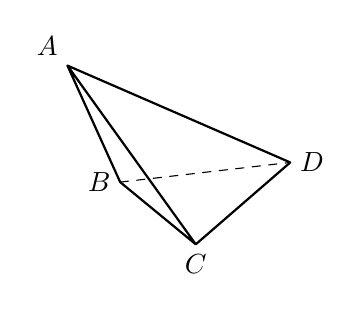
\begin{tikzpicture}[line cap=round,line join=round,scale=1.0]
  \coordinate (A) at (-1.45,1.95);
  \coordinate (B) at (-0.78,0.47);
  \coordinate (C) at (0.18,-0.32);
  \coordinate (D) at (1.38,0.72);

  % 原图中 BD 为隐藏棱，其余外轮廓与侧棱为实线。
  \draw[thick] (A)--(B) (A)--(C) (A)--(D) (B)--(C) (C)--(D);
  \draw[dashed] (B)--(D);

  \node[above left] at (A) {$A$};
  \node[left] at (B) {$B$};
  \node[below] at (C) {$C$};
  \node[right] at (D) {$D$};
\end{tikzpicture}
